\chapter{Fundamentals of OSGi}

\section{An overview of architecture}
The OSGi framework's specification defines three conceptual layers, figure ~\ref{fig:layers}
\begin{figure}
	\centering
		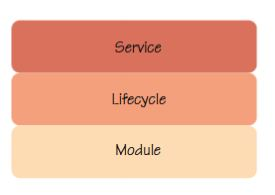
\includegraphics{image/layers.JPG}
	\caption{Three layers OSGi architecture }
	\label{fig:layers}
\end{figure}
 
\begin{itemize}
	\item \textbf{\textit{Module Layer}} - Concerned with packing and sharing code
	\item \textbf{\textit{Lifecyle Layer}} - Concerned with managing modules
	\item \textbf{\textit{Module Layer}} - Concerned with interaction and communication among modules
\end{itemize}
Each layer is dependent on the layers beneath it.
\section{Module Layer}
The module layer defines the OSGi module concept. An OSGi module is terminologically called\textit{a bundle}
\subsection{OSGi bundles}
Basically, OSGi bundles are JAR files with extra meta-data. A bundle consist of Java classes, a meta-data file called MANIFEST in which every information related to the bundle is clearly defined, other resources like xml files or images are also packed into a bundle, figure ~\ref{fig:bundle}
\begin{figure}
	\centering
		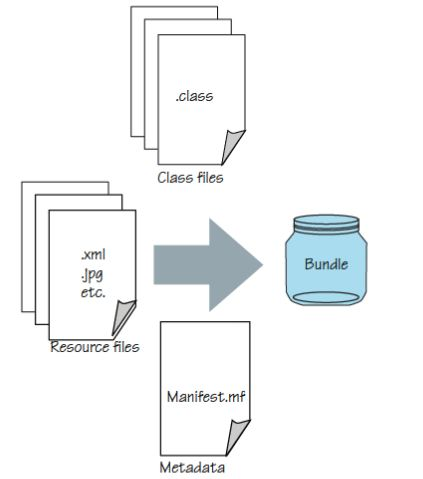
\includegraphics{image/bundle.JPG}
	\caption{An OSGi bundle's composition}
	\label{fig:bundle}
\end{figure}

OSGi bundles are more powerful than normal JAR files because they are able to explicitly declare which internal packages are externally visible, exported packages. With standard Java, only classes have this mechanism by using keywords public, private or protected to indicate which class members can be used from outside classes, or which classes from one package are visible to others. Additionally, since a bundle always has a specific version, defined in MANIFEST file, all exposed packages are accompanied by the version of the bundle that they are from.

On the other hand, when a bundle needs to use code from other bundles, it also explicitly declares which packages with a specific version or a range of version must be provided, these packages are called imported packages. As long as the right code versions are unsatisfied, the bundle will not be able to deploy correctly. 
\begin{figure}
	\centering
		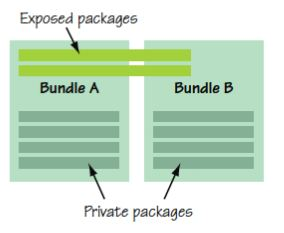
\includegraphics{image/packages.JPG}
	\caption{Exposed packages from Bundle A are visible to Bundle B, while unexposed packages are private}
	\label{fig:packages}
\end{figure}

The main benefit of explicitly declaring imported packages and exported packages for bundles is that the consistency of their versions is managed and verified automatically by the OSGi framework; hence, code versions are always guaranteed to be consistent before code is executed at run-time, which cannot be ensured with Java class path.

\subsection{Bundle meta-data}
All information of a bundle is included in the MANIFEST file. Normally, the MANIFEST file stores basic information about version, name, exported and imported packages of a bundle.
    


\section{Life-cycle layer}
bundle life-cycle

\section{Service layer}

\subsection{Publishing services}
\subsection{Consuming services}

\section{Bundle activation}
\subsection{Bundle activator}
\subsection{Blue-print framework}

\section{Typical architecture of OSGi-based applications}




 
